% !TeX root = ba.tex

\section{Experiments}

\subsection{Datasets and Network Architectures}

\subsection{Results}

\todo{Nicer looking tables}
\begin{table*}[h]
%	\begin{minipage}{.45\linewidth}
		\caption{Average perturbation norms for each attack and architecture.}
		\vskip 0.15in
		\centering\scalebox{1.0}{
			\begin{tabular}{llcccc}
				\toprule
				Attack & Network       & MNIST & Fashion & SVHN & CIFAR10  \\
				\midrule
				\multirow{2}{*}{CW} & ConvNet & {$1.40$} & $0.51$ & $0.67$ & $0.37$ \\
				& CapsNet            & $1.82$ & {$0.50$} & {$0.60$} & {$0.23$} \\
				\midrule
				\multirow{2}{*}{Boundary} & ConvNet & {$3.07$} & $1.24$ & $2.42$ & $1.38$ \\
				& CapsNet            & $3.26$ & {$0.93$} & {$1.88$} & {$0.72$} \\
				\midrule
				\multirow{2}{*}{DeepFool} & ConvNet & {$1.07$} & {$0.31$} & {$0.41$} & $0.23$ \\
				& CapsNet           & $2.02$ & $0.55$ & $0.80$ & {$0.16$} \\
				\midrule
				\multirow{2}{*}{Universal} & ConvNet & {$6.71$} & {$2.61$} & {$2.46$} & {$2.45$} \\
				& CapsNet           & $11.45$ & $5.31$ & $8.59$ & $2.70$ \\
				\bottomrule\\
		\end{tabular}}
		\label{tab:norms}
		
%	\end{minipage}\hspace{0.8cm}
%	\begin{minipage}{.45\linewidth}
		\caption{Fooling rates of adversarial examples calculated for a CapsNet and evaluated on a ConvNet and vice versa. For the universal attack we report the accuracy on the whole test set.}
		\vskip 0.15in
		\centering\scalebox{1.0}{
			\begin{tabular}{llcccc}
				\toprule
				Attack & Network       & MNIST & Fashion & SVHN & CIFAR10  \\
				\midrule
				\multirow{2}{*}{CW} & ConvNet & $0.8\%$ & $1.2\%$ & $2.8\%$ & $2.4\%$ \\
				& CapsNet            & $2.0\%$ & $2.0\%$ & $3.8\%$ & $2.0\%$ \\
				\midrule
				\multirow{2}{*}{Boundary} & ConvNet & $8.8\%$ & $9.5\%$ & $10.5\%$ & $13.4\%$ \\
				& CapsNet            & $14.2\%$ & $14.6\%$ & $12.9\%$ & $26.1\%$ \\
				\midrule
				\multirow{2}{*}{DeepFool} & ConvNet & $4.3\%$ & $8.5\%$ & $13.5\%$ & $11.8\%$ \\
				& CapsNet           & $0.9\%$ & $10.9\%$ & $10.8\%$ & $14.1\%$ \\
				\midrule
				\multirow{2}{*}{Universal} & ConvNet & $4.9\%$ & $20.4\%$ & $35.0\%$ & $25.9\%$ \\
				& CapsNet           & $38.2\%$ & $25.7\%$ & $53.4\%$ & $47.2\%$ \\
				\bottomrule\\
		\end{tabular}}
		\label{tab:attacks}%\end{minipage}
\end{table*}

\subsection{Difference between Adversarial Examples}
\subsubsection{Universal Attack T-SNE}

We used T-SNE \citep{tsne} to make a scatter plot.
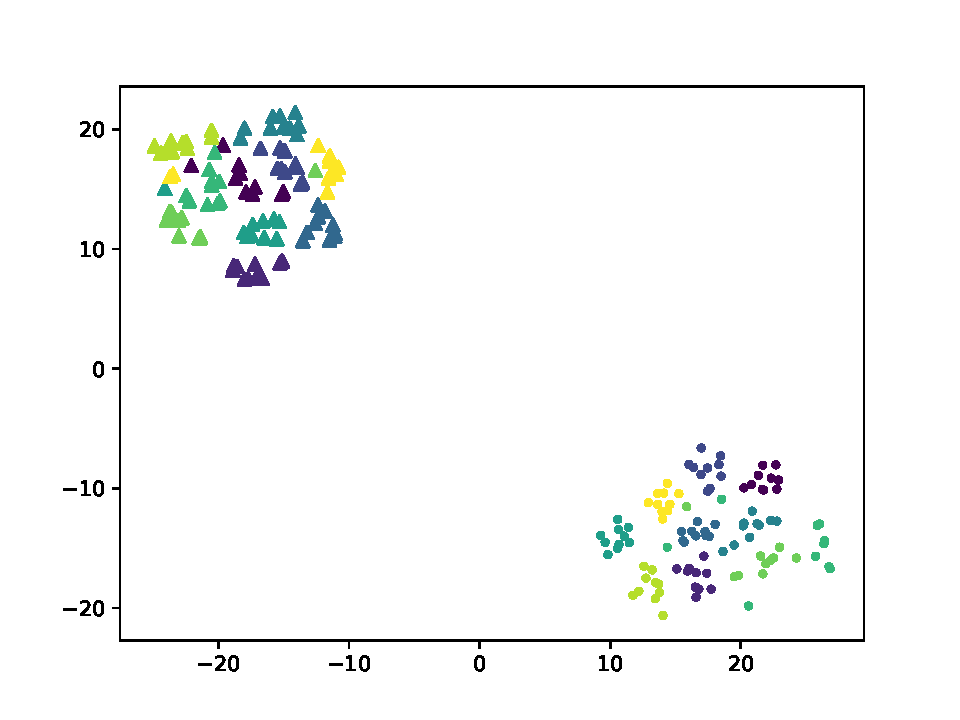
\includegraphics[height=7cm]{tsne.pdf}

\subsubsection{SVD}

\citet{universal} considered singular values of the matrix containing normalized adversarial examples to determine, if adversarial examples lie in a low dimensional subspace. \\
For this purpose, let us denote with $\delta(x)$ the minimal adversarial perturbation for the input $x \in [0,1]^n$,
and $ N = \begin{bmatrix}
\frac{\delta(x_1)} {\norm{\delta(x_1)}},  ...,  \frac{\delta(x_k)} {\norm{\delta(x_k)}} 
\end{bmatrix}
\in \mathrm{R}^{n \times k}
$ for some $x_1, ..., x_k$ in the test set. \\
$\delta(x)$ is orthogonal to the decision boundary, assuming it is reasonably smooth, therefore the singular values of N give us information about the decision boundary. For example, for an binary linear classifier, N would have a rank of one, i.e. only one non-zero singular value.

In this regard we find little difference between CapsNets and CNNs.